
\documentclass[xcolor=dvipsnames]{beamer}  % for hardcopy add 'trans'

\mode<presentation>
{
  \usetheme{Singapore}
  % or ...
  \setbeamercovered{transparent}
  % or whatever (possibly just delete it)
}

\usefonttheme{professionalfonts}
%\usepackage[english]{babel}
% or whatever
%\usepackage[latin1]{inputenc}
% or whatever
%\usepackage{times}
%\usepackage[T1]{fontenc}
% Or whatever. Note that the encoding and the font should match. If T1
% does not look nice, try deleting the line with the fontenc.

%%%%%%%%%%%%%%%%%%%%%% start my preamble %%%%%%%%%%%%%%%%%%%%%%


\addtobeamertemplate{navigation symbols}{}{%
    \usebeamerfont{footline}%
    \usebeamercolor[fg]{footline}%
    \hspace{1em}%
    \insertframenumber/\inserttotalframenumber
}

\setbeamercolor{footline}{fg=blue}
\setbeamerfont{footline}{series=\bfseries}


%\usepackage{epsfig}
\usepackage{graphicx}
\usepackage{amsmath, amssymb, amsthm}

\usepackage{fancyvrb}

\usepackage{tikz}
\usetikzlibrary{arrows}
\usetikzlibrary{calc}
\usetikzlibrary{intersections}
\usetikzlibrary{decorations}
\usepackage{pgf}
\usepackage{pgfplots}
\pgfplotsset{compat=1.13}

\usepackage{graphviz}
 
\usepackage{verbatim}


\usepackage{algorithmicx,algpseudocode}


%font
\usepackage{mathpazo}
%\usepackage[usenames, dvipsnames]{color}

%\usepackage[linesnumbered, ruled, lined]{algorithm2e}

\usepackage{xr}
\externaldocument[ET-]{et}


\newcommand*{\theorembreak}{\usebeamertemplate{theorem end}\framebreak\usebeamertemplate{theorem begin}}

\newcommand{\newtopic}[1]{\textcolor{Green}{\Large \bf #1}}
\newcommand{\navy}[1]{\textcolor{Blue}{\bf #1}}
\newcommand{\navymth}[1]{\textcolor{Blue}{#1}}
\newcommand{\red}[1]{\textcolor{red}{#1}}


\definecolor{pale}{RGB}{235, 235, 235}
\definecolor{pale2}{RGB}{175,238,238}
\definecolor{turquois4}{RGB}{0,134,139}

% Typesetting code
\definecolor{bg}{rgb}{0.95,0.95,0.95}
\usepackage{minted}
\usemintedstyle{friendly}
\newminted{python}{mathescape,frame=lines,framesep=4mm,bgcolor=bg}
\newminted{ipython}{mathescape,frame=lines,framesep=4mm,bgcolor=bg}
\newminted{julia}{mathescape,frame=lines,framesep=4mm,bgcolor=bg}
\newminted{c}{mathescape,linenos=true}
\newminted{r}{mathescape,  frame=none, baselinestretch=1, framesep=2mm}
\renewcommand{\theFancyVerbLine}{\sffamily
    \textcolor[rgb]{0.5,0.5,1.0}{\scriptsize {\arabic{FancyVerbLine}}}}


\usepackage{stmaryrd}

\newcommand{\Fact}{\textcolor{Brown}{\bf Fact. }}
\newcommand{\Facts}{\textcolor{Brown}{\bf Facts }}
\newcommand{\keya}{\textcolor{turquois4}{\bf Key Idea. }}
\newcommand{\Factnodot}{\textcolor{Brown}{\bf Fact }}
\newcommand{\Eg}{\textcolor{ForestGreen}{Example. }}
\newcommand{\Egs}{\textcolor{ForestGreen}{Examples. }}
\newcommand{\Ex}{{\bf Ex. }}
\newcommand{\Thm}{\textcolor{Brown}{\bf Theorem. }}
\newcommand{\Prf}{\textcolor{turquois4}{\bf Proof.}}
\newcommand{\Ass}{\textcolor{turquois4}{\bf Assumption.}} 
\newcommand{\Lem}{\textcolor{Brown}{\bf Lemma. }}

%source code 



% caligraphic
\usepackage{mathrsfs}
\usepackage{bbm}
\usepackage{subfigure}

\newcommand{\argmax}{\operatornamewithlimits{argmax}}
\newcommand{\argmin}{\operatornamewithlimits{argmin}}

\newcommand\T{{\mathpalette\raiseT\intercal}}
\newcommand\raiseT[2]{\raisebox{0.25ex}{$#1#2$}}

\DeclareMathOperator{\cl}{cl}
%\DeclareMathOperator{\argmax}{argmax}
\DeclareMathOperator{\interior}{int}
\DeclareMathOperator{\Prob}{Prob}
\DeclareMathOperator{\kernel}{ker}
\DeclareMathOperator{\diag}{diag}
\DeclareMathOperator{\sgn}{sgn}
\DeclareMathOperator{\determinant}{det}
\DeclareMathOperator{\trace}{trace}
\DeclareMathOperator{\Span}{span}
\DeclareMathOperator{\rank}{rank}
\DeclareMathOperator{\cov}{cov}
\DeclareMathOperator{\corr}{corr}
\DeclareMathOperator{\range}{rng}
\DeclareMathOperator{\var}{var}
\DeclareMathOperator{\mse}{mse}
\DeclareMathOperator{\se}{se}
\DeclareMathOperator{\row}{row}
\DeclareMathOperator{\col}{col}
\DeclareMathOperator{\dimension}{dim}
\DeclareMathOperator{\fracpart}{frac}
\DeclareMathOperator{\proj}{proj}
\DeclareMathOperator{\colspace}{colspace}

\providecommand{\inner}[1]{\left\langle{#1}\right\rangle}

% mics short cuts and symbols
% mics short cuts and symbols
\newcommand{\st}{\ensuremath{\ \mathrm{s.t.}\ }}
\newcommand{\setntn}[2]{ \{ #1 : #2 \} }
\newcommand{\cf}[1]{ \lstinline|#1| }
\newcommand{\otms}[1]{ \leftidx{^\circ}{#1}}

\newcommand{\fore}{\therefore \quad}
\newcommand{\tod}{\stackrel { d } {\to} }
\newcommand{\tow}{\stackrel { w } {\to} }
\newcommand{\toprob}{\stackrel { p } {\to} }
\newcommand{\toms}{\stackrel { ms } {\to} }
\newcommand{\eqdist}{\stackrel {\textrm{ \scriptsize{d} }} {=} }
\newcommand{\iidsim}{\stackrel {\textrm{ {\sc iid }}} {\sim} }
\newcommand{\1}{\mathbbm 1}
\newcommand{\dee}{\,{\rm d}}
\newcommand{\given}{\, | \,}
\newcommand{\la}{\langle}
\newcommand{\ra}{\rangle}

\renewcommand{\rho}{\varrho}

\newcommand{\htau}{ \hat \tau }
\newcommand{\hgamma}{ \hat \gamma }

\newcommand{\boldx}{ {\mathbf x} }
\newcommand{\boldu}{ {\mathbf u} }
\newcommand{\boldv}{ {\mathbf v} }
\newcommand{\boldw}{ {\mathbf w} }
\newcommand{\boldy}{ {\mathbf y} }
\newcommand{\boldb}{ {\mathbf b} }
\newcommand{\bolda}{ {\mathbf a} }
\newcommand{\boldc}{ {\mathbf c} }
\newcommand{\boldi}{ {\mathbf i} }
\newcommand{\bolde}{ {\mathbf e} }
\newcommand{\boldp}{ {\mathbf p} }
\newcommand{\boldq}{ {\mathbf q} }
\newcommand{\bolds}{ {\mathbf s} }
\newcommand{\boldt}{ {\mathbf t} }
\newcommand{\boldz}{ {\mathbf z} }

\newcommand{\boldzero}{ {\mathbf 0} }
\newcommand{\boldone}{ {\mathbf 1} }

\newcommand{\boldalpha}{ {\boldsymbol \alpha} }
\newcommand{\boldbeta}{ {\boldsymbol \beta} }
\newcommand{\boldgamma}{ {\boldsymbol \gamma} }
\newcommand{\boldtheta}{ {\boldsymbol \theta} }
\newcommand{\boldxi}{ {\boldsymbol \xi} }
\newcommand{\boldtau}{ {\boldsymbol \tau} }
\newcommand{\boldepsilon}{ {\boldsymbol \epsilon} }
\newcommand{\boldmu}{ {\boldsymbol \mu} }
\newcommand{\boldSigma}{ {\boldsymbol \Sigma} }
\newcommand{\boldOmega}{ {\boldsymbol \Omega} }
\newcommand{\boldPhi}{ {\boldsymbol \Phi} }
\newcommand{\boldLambda}{ {\boldsymbol \Lambda} }
\newcommand{\boldphi}{ {\boldsymbol \phi} }

\newcommand{\Sigmax}{ {\boldsymbol \Sigma_{\boldx}}}
\newcommand{\Sigmau}{ {\boldsymbol \Sigma_{\boldu}}}
\newcommand{\Sigmaxinv}{ {\boldsymbol \Sigma_{\boldx}^{-1}}}
\newcommand{\Sigmav}{ {\boldsymbol \Sigma_{\boldv \boldv}}}

\newcommand{\hboldx}{ \hat {\mathbf x} }
\newcommand{\hboldy}{ \hat {\mathbf y} }
\newcommand{\hboldb}{ \hat {\mathbf b} }
\newcommand{\hboldu}{ \hat {\mathbf u} }
\newcommand{\hboldtheta}{ \hat {\boldsymbol \theta} }
\newcommand{\hboldtau}{ \hat {\boldsymbol \tau} }
\newcommand{\hboldmu}{ \hat {\boldsymbol \mu} }
\newcommand{\hboldbeta}{ \hat {\boldsymbol \beta} }
\newcommand{\hboldgamma}{ \hat {\boldsymbol \gamma} }
\newcommand{\hboldSigma}{ \hat {\boldsymbol \Sigma} }

\newcommand{\boldA}{\mathbf A}
\newcommand{\boldB}{\mathbf B}
\newcommand{\boldC}{\mathbf C}
\newcommand{\boldD}{\mathbf D}
\newcommand{\boldI}{\mathbf I}
\newcommand{\boldL}{\mathbf L}
\newcommand{\boldM}{\mathbf M}
\newcommand{\boldP}{\mathbf P}
\newcommand{\boldQ}{\mathbf Q}
\newcommand{\boldR}{\mathbf R}
\newcommand{\boldX}{\mathbf X}
\newcommand{\boldU}{\mathbf U}
\newcommand{\boldV}{\mathbf V}
\newcommand{\boldW}{\mathbf W}
\newcommand{\boldY}{\mathbf Y}
\newcommand{\boldZ}{\mathbf Z}

\newcommand{\bSigmaX}{ {\boldsymbol \Sigma_{\hboldbeta}} }
\newcommand{\hbSigmaX}{ \mathbf{\hat \Sigma_{\hboldbeta}} }

\newcommand{\RR}{\mathbbm R}
\newcommand{\CC}{\mathbbm C}
\newcommand{\NN}{\mathbbm N}
\newcommand{\PP}{\mathbbm P}
\newcommand{\EE}{\mathbbm E \nobreak\hspace{.1em}}
\newcommand{\EEP}{\mathbbm E_P \nobreak\hspace{.1em}}
\newcommand{\ZZ}{\mathbbm Z}
\newcommand{\QQ}{\mathbbm Q}


\newcommand{\XX}{\mathcal X}

\newcommand{\aA}{\mathcal A}
\newcommand{\fF}{\mathscr F}
\newcommand{\bB}{\mathscr B}
\newcommand{\iI}{\mathscr I}
\newcommand{\rR}{\mathscr R}
\newcommand{\dD}{\mathcal D}
\newcommand{\lL}{\mathcal L}
\newcommand{\llL}{\mathcal{H}_{\ell}}
\newcommand{\gG}{\mathcal G}
\newcommand{\hH}{\mathcal H}
\newcommand{\nN}{\textrm{\sc n}}
\newcommand{\lN}{\textrm{\sc ln}}
\newcommand{\pP}{\mathscr P}
\newcommand{\qQ}{\mathscr Q}
\newcommand{\xX}{\mathcal X}

\newcommand{\ddD}{\mathscr D}


\newcommand{\R}{{\texttt R}}
\newcommand{\risk}{\mathcal R}
\newcommand{\Remp}{R_{{\rm emp}}}

\newcommand*\diff{\mathop{}\!\mathrm{d}}
\newcommand{\ess}{ \textrm{{\sc ess}} }
\newcommand{\tss}{ \textrm{{\sc tss}} }
\newcommand{\rss}{ \textrm{{\sc rss}} }
\newcommand{\rssr}{ \textrm{{\sc rssr}} }
\newcommand{\ussr}{ \textrm{{\sc ussr}} }
\newcommand{\zdata}{\mathbf{z}_{\mathcal D}}
\newcommand{\Pdata}{P_{\mathcal D}}
\newcommand{\Pdatatheta}{P^{\mathcal D}_{\theta}}
\newcommand{\Zdata}{Z_{\mathcal D}}




\newcommand{\e}[1]{\mathbbm{E}[{#1}]}
\newcommand{\p}[1]{\mathbbm{P}({#1})}

%\theoremstyle{plain}
%\newtheorem{axiom}{Axiom}[section]
%\newtheorem{theorem}{Theorem}[section]
%\newtheorem{corollary}{Corollary}[section]
%\newtheorem{lemma}{Lemma}[section]
%\newtheorem{proposition}{Proposition}[section]
%
%\theoremstyle{definition}
%\newtheorem{definition}{Definition}[section]
%\newtheorem{example}{Example}[section]
%\newtheorem{remark}{Remark}[section]
%\newtheorem{notation}{Notation}[section]
%\newtheorem{assumption}{Assumption}[section]
%\newtheorem{condition}{Condition}[section]
%\newtheorem{exercise}{Ex.}[section]
%\newtheorem{fact}{Fact}[section]

% Bibliography
\usepackage[authordate,uniquename=false,firstinits,backend=biber,maxcitenames=2]{biblatex-chicago}
\DeclareFieldFormat[article]{title}{#1}
\DeclareFieldFormat[inproceedings]{title}{#1}
\addbibresource{et_newbib.bib}
\renewcommand{\cite}{\textcite}



\setlength{\parskip}{1.5ex plus0.5ex minus0.5ex}


\setlength{\jot}{12pt} 









\title{A Primer in Econometric Theory}

\subtitle
{Lecture 10:  Regression}

\author{John Stachurski \\ \tiny Lectures by Akshay Shanker}



\begin{document}

\begin{frame}
  \titlepage
\end{frame}

\section{Linear Regression}


\begin{frame}\frametitle{Linear Regression}
    
    \vspace{2em}
    Start with the prediction problem discussed in \S\ref{ET-ss:erm} --- a system with vector input $\boldx_n \in \RR^K$ followed by scalar
    output $y_n$
    
    \vspace{.7em}
    Examples:
    
    \begin{itemize}
        \item $\boldx_n$ is a description of a lottery (probabilities,
            possible outcomes, etc.) 
            in a controlled experiment and $y_n$ is willingness to pay in order to
            participate 
        \item $\boldx_n$ is a set of household characteristics (ethnicity,
        age, location, etc.) and $y_n$ is household wealth at some later
            date 
        \item $\boldx_n$ is price of electricity, prices of alternatives,
            temperature, household income, and measurements of the regional income
            distribution, while $y_n$ is regional electricity consumption 
    \end{itemize}
    
\end{frame}

\begin{frame}

    \vspace{2em}
    Suppose we have $N$ observations $\boldz_n := (\boldx_n,y_n)$, 
    all draws from fixed joint distribution $P$
    
    Since $P$ is fixed, we are assuming the system is stationary across the set of draws
     
    \vspace{.7em}     
    Our problem:
    %
    \small\begin{equation*}\label{eq:prp}
        \text{choose function } f \colon \RR^K \to \RR \text{ such that }
        f(\boldx) \text{ is a good predictor of } y
    \end{equation*}
 
\end{frame}

\begin{frame}
     
    \vspace{2em}
    To define ``good predictor" mathematically, we need a loss function
    
    We will be using quadratic loss, thus minimize
    the prediction risk given by
    %
    \begin{equation}
        \label{eq:rf2}
        R(f) := \EEP  (y - f(\boldx))^2 
    \end{equation}
    
    \vspace{.7em}
    Minimizer of \eqref{eq:rf2} over the
    set of all $\bB$-measurable functions is the regression
    function $f^*(\boldx) :=
    \EEP  [y \given \boldx]$
    
    Recall we cannot compute the regression function because $P$ is not known 
    
\end{frame}

\begin{frame}

    \vspace{2em}
    Instead we apply the principle of empirical risk minimization,
    which leads to the problem
    %
    \begin{equation}
        \label{eq:ermm}
        \min_{f \in \hH} \Remp(f)
        \quad \text{where} \quad
        \Remp(f) := \frac{1}{N} \sum_{n=1}^N (y_n - f(\boldx_n))^2
    \end{equation}
    
    \vspace{.7em}
    Here $\hH$ is the hypothesis space, a set of candidate functions 
    mapping $\RR^K$ into $\RR$
    
    The problem \eqref{eq:ermm} is
    called a \navy{least squares} problem
  
\end{frame}

\begin{frame}

    \vspace{2em}
    As discussed at length in \S\ref{ET-ss:ermls},
    minimizing empirical risk is different from minimizing the prediction risk
    $R(f)$ --- thus $\hH$ must be
    restricted 
    
    \vspace{.7em}
    Consider the case $\hH = \llL$, where $\llL$ is all
    linear functions from $\RR^K$ to $\RR$
    
    Recalling theorem~\ref{ET-t:lmaeq}, write
    %
    \begin{equation*}
        \label{eq:allaff2}
        \llL = 
        \left\{ \, \text{all } f \colon \RR^K \to \RR \, 
            \text{ such that }
            f(\boldx) = \boldx^\T \boldb \text{ for some } \boldb \in \RR^K 
        \right\}
    \end{equation*}
    
    
    Problem \eqref{eq:ermm} reduces to 
    %
    \begin{equation}
        \label{eq:olslq}
            \min_{\boldb \in \RR^K} \;
            \sum_{n=1}^N (y_n - \boldx_n^\T \boldb)^2
    \end{equation}
    
\end{frame}

\begin{frame}

    \vspace{2em}
    Intuition: ``line of best fit" to minimize in-sample prediction error
    
    \vspace{.7em}
    Good reasons to start with $\llL$, even where no linearity
    assumptions are imposed:
    
    \begin{enumerate}
        \item $\llL$ is a natural starting point when
            seeking a class of simple, well-behaved functions
        \item setting $\hH
            = \llL$ allows us to obtain an analytical expression for the minimizer, 
            which simplifies both analysis and computation
        \item the technique has an extension from
            $\llL$ to broader classes of functions
    \end{enumerate}

\end{frame}

\begin{frame}\frametitle{Least Squares Estimator}

    \vspace{2em}
    Now let's solve \eqref{eq:olslq}. Let 
    %
    \small \begin{equation*}
        \label{eq:design0}
        \boldy := 
        \left(
        \begin{array}{c}
            y_1 \\
            y_2 \\
            \vdots \\
            y_N
        \end{array}
        \right),\,
        \boldx_n := 
        \left(
        \begin{array}{c}
            x_{n1} \\ 
            x_{n2} \\
            \vdots \\
            x_{nK}
        \end{array}
        \right)
        = \text{ $n$th observation of all regressors}
    \end{equation*}
    %
    and
    %
    \small \begin{equation*}
        \label{eq:design}
        \boldX := 
        \left(
        \begin{array}{c}
            \boldx_1^\T  \vspace{0.2em}  \\
            \boldx_2^\T  \\
            \vdots     \\
            \boldx_N^\T  
        \end{array}
        \right)
        :=:
        \left(
        \begin{array}{cccc}
            x_{11} & x_{12} & \cdots & x_{1K} \\
            x_{21} & x_{22} & \cdots & x_{2K} \\
            \vdots & \vdots &  & \vdots \\
            x_{N1} & x_{N2} & \cdots & x_{NK} 
        \end{array}
        \right)
    \end{equation*}
    
\end{frame}

\begin{frame}

    \vspace{2em}
    Sometimes $\boldX$ is called the \navy{design matrix}
    
    By construction, $\col_k \boldX =$ all observations on the $k$th regressor
    
    \vspace{.7em}
    Also, for any $\boldb \in \RR^K$, we have
    %
    \begin{equation*}
        \boldX \boldb = 
        \left(
        \begin{array}{c}
            \boldx_1^\T \boldb \vspace{0.2em} \\
            \boldx_2^\T \boldb\\
            \vdots \\
            \boldx_N^\T \boldb
        \end{array}
        \right)
    \end{equation*}
%
\end{frame}

\begin{frame}

    \vspace{2em}
    The objective function in (\ref{eq:olslq}) can be written as 
    %
    \begin{equation*}
         \sum_{n=1}^N (y_n - \boldx_n^\T \boldb)^2 
            = \| \boldy - \boldX \boldb \|^2
    \end{equation*}
    %
    Since strictly increasing transforms preserve the set of minimizers 
    %
    \begin{equation}
        \label{eq:olses}
        \argmin_{\boldb \in \RR^K} \| \boldy - \boldX \boldb \|^2
         = \argmin_{\boldb \in \RR^K} \| \boldy - \boldX \boldb \|
    \end{equation}
    
    Using the orthogonal projection theorem (recall theorem~\ref{ET-t:lssol} in ET), the
    solution is
    %
    \begin{equation}
        \label{eq:thelsqe}
        \hboldbeta := (\boldX^\T \boldX)^{-1} \boldX^\T \boldy
    \end{equation}
\end{frame}

\begin{frame}
    
    \vspace{2em}
    Traditionally, $\hboldbeta$ called the \navy{least
    squares estimator}
    
    Once we move to more classical assumptions it 
    will be an estimator of a particular parameter vector
    
    \vspace{.7em}
    At this stage it just
    defines our answer to the problem posed in \eqref{eq:prp}.  That is,
    %
    \begin{equation*}
        \text{given $\boldx \in \RR^K$, our prediction of $y$ is }
        f(\boldx) = \boldx^\T \hboldbeta
    \end{equation*}
    
\end{frame}

\begin{frame}
    
    \vspace{2em}
    In terms of geometric interpretation, since $\boldX \hboldbeta$ solves
    \eqref{eq:olses}, it is the closest point in $\colspace \boldX$
    to $\boldy$:
    %
    \begin{equation*}
        \boldP \boldy = \boldX \hboldbeta   
        \quad \text{when} \quad
        \boldP := \proj \, (\colspace \boldX )
    \end{equation*}
    
    \vspace{.7em}
    In what follows,
    $\boldM$ is the residual projection, as defined in \eqref{ET-eq:ann0} in ET

\end{frame}

\begin{frame}\frametitle{Assumptions}
 
    \vspace{2em}
    \Ass\eqref{ET-a:fr} 
    $\boldX$ has full column rank with probability one
      
    By theorem~\ref{ET-t:exth}, $N \geq K$ is a necessary
    condition for the assumption to hold
    
    (If $N < K$, then $\RR^N$, which
    is necessarily spanned by $N$ vectors, cannot contain $K$ linearly
    independent vectors)
    
    \vspace{.7em}
    If this assumption does not hold, then minimizer of \eqref{eq:olses} still exists
    but is no longer unique (see ex.~\ref{ET-ex:lsiosol})  
    
\end{frame}

\begin{frame}
  
    \vspace{2em}
    \Ass\eqref{ET-a:poprank}
    $P$ is such that all elements of $\EE_P [ \boldz_n \boldz_n^\T]$ are finite. 
    Moreover
    %
    \begin{equation}
        \label{eq:smx}
        \Sigmax := \EE_P [ \boldx_n \boldx_n^\T ] \; \text{ is finite and positive definite}
    \end{equation}

    \vspace{.7em}
    Finite second moments imposed to evaluate expected squared errors 
    
    Assumption cannot be weakened unless we are willing to work with a 
    different loss function
\end{frame}

\begin{frame}\frametitle{Notation}
    
    \vspace{2em}
    The projection
    %
    \begin{equation*}
        \hboldy := \boldX \hboldbeta = \boldP \boldy
    \end{equation*}
    %
    is called the \navy{vector of fitted values}
    
    The $n$th fitted value $\hat
    y_n$ is the prediction $\boldx_n^\T \, \hboldbeta$ associated with least
    squares estimate
    and the $n$th observation $\boldx_n$ of the input vector
    
    \vspace{.7em}
    The vector $\boldM
    \boldy$ is often denoted $\hboldu$, and called the \navy{vector of residuals}:
    %
    \begin{equation*}
        \hboldu := \boldM \boldy = \boldy - \hboldy
    \end{equation*}
    %
\end{frame}

\begin{frame}

    \vspace{2em}
    The vector of residuals corresponds to the error that occurs when $\boldy$ is
    approximated by $\boldP \boldy$
    
    From fact~\ref{ET-fa:opt3}
    %
    \begin{equation}
        \label{eq:orr}
        \boldM \boldy \perp \boldP \boldy 
        \quad \text{and} \quad 
        \boldy =  \boldP \boldy + \boldM \boldy
    \end{equation}
    
    \vspace{.7em}
    In other words, $\boldy$ can be decomposed into two orthogonal vectors $\boldP
    \boldy$ and $\boldM \boldy$:
    \begin{itemize}
        \item first represents the best approximation
    to $\boldy$ in $\colspace \boldX$
        \item second represents the residual
    \end{itemize}

\end{frame}

\begin{frame}
    
    \vspace{2em}
    Related to the fitted values and residuals, we have some standard definitions:
    %
    \begin{itemize}
        \item \navy{Total sum of squares} $:= \tss := \| \boldy \|^2$
        \item \navy{Residual sum of squares} $ := \rss := \| \boldM \boldy \|^2$
        \item \navy{Explained sum of squares} $ := \ess := \| \boldP \boldy \|^2$
    \end{itemize}
    %
    By (\ref{eq:orr}) and the Pythagorean law
    %
    \begin{equation}
        \label{eq:bdtss}
        \tss = \ess + \rss
    \end{equation}
    
    \vspace{.7em}
    When running regressions it is conventional to report the \navy{coefficient
    of determination}, or $R^2$:
    %
    \begin{equation}
        \label{eq:rsd}
        R^2 := \frac{\ess}{\tss}
    \end{equation}
    %
\end{frame}


\begin{frame}\frametitle{Out of Sample Fit}
    
    \vspace{2em}
    How does linear least squares perform out-of-sample? Start with
    a general
    observation:

    \Thm
        \eqref{ET-t:dclee}
        If $\ell$ is the linear function $\ell (\boldx) =
        \boldx^\T \boldb$, then
        %
        \begin{multline*}
            R(\ell)
            = \EE (y - f^*(\boldx))^2  
           \\ + \EE (f^*(\boldx) - \boldx^\T \boldb^*)^2 
            +  (\boldb^* - \boldb)^\T 
                \Sigmax (\boldb^* - \boldb) 
        \end{multline*}
        %
    
    Here $f^*$ is the regression function and $\boldb^* = \Sigmax^{-1} \,
    \EE[\boldx \, y]$ is the vector of coefficients in the best linear predictor
    
    $R(f)$ is the prediction risk
    of $f$ and expectations are taken under the unknown joint distribution $P$ of
    the pairs $(\boldx, y)$

\end{frame}

\begin{frame}
    
    \vspace{2em}
    Theorem~\ref{ET-t:dclee} decomposes the prediction risk of an
    arbitrary linear predictor $\ell (\boldx) = \boldx^\T \boldb$
    into three terms:
    %
    \begin{enumerate}
        \label{enum:tr}
        \item The \navy{intrinsic risk} $\EE (y - f^*(\boldx))^2 $
        \item The \navy{approximation error} $\EE (f^*(\boldx) - \boldx^\T
            \boldb^*)^2 $
        \item The \navy{estimation error} $ (\boldb^* - \boldb)^\T 
        \Sigmax (\boldb^* - \boldb)$
    \end{enumerate}

\end{frame}
  
 \begin{frame}
    
    \vspace{2em}
    The intrinsic risk is also called Bayes risk, it is the residual error after $y$ 
    is approximated with the best possible predictor
    \begin{itemize}
        \item large to the extent
        that $y$ is hard to predict using $\boldx$
    \end{itemize}
    
    \vspace{.7em}
    The approximation error or \emph{bias} is the deviation between the best
    predictor and the best linear predictor

\end{frame}

\begin{frame}

    \vspace{2em}
    The estimation error is caused by the deviation of our estimator
    from the best linear predictor $\boldb^*$
    \begin{itemize}
        \item deviation occurs because
    we are predicting using finite sample information on the joint
    distribution of $(\boldx, y)$
    \end{itemize}
    
\end{frame}

\begin{frame}

    \vspace{2em}
    \Thm\eqref{ET-t:cwa}
    Let assumptions~\ref{ET-a:poprank}--\ref{ET-a:fr} hold and let $\hboldbeta_N$ be
    the least squares estimator given sample size $N$.  If the observations
    $\{\boldz_n\}$ are independent,  then
    %
    \begin{equation}
        \label{eq:cwa}
        \hboldbeta_N \; \toprob \; \boldb^*
          \quad \text{as} \quad
        N \to \infty
    \end{equation}
    %
    
    \vspace{.7em}
    Independence required only for the LLN to function --- can weaken to ergodicity
    
\end{frame}


\begin{frame}\frametitle{Proofs}

    \vspace{2em}
    \Prf[Proof of theorem~\ref{ET-t:dclee}]
        Fix $\boldb \in \RR^K$ and let 
        $\ell (\boldx) =
        \boldx^\T \boldb$
        
        Recall from
        \eqref{ET-eq:ebrf2} in ET that we can write the
        the prediction risk as
        %
        \begin{equation*}
            R(\ell)
            = \EE[ (y - f^*(\boldx))^2 ] 
            + \EE[ (f^*(\boldx) - \boldx^\T \boldb)^2 ]
        \end{equation*}
        %
        To establish result, we show
        %
        \begin{multline}
            \label{eq:odbb}
            \EE[ (f^*(\boldx) - \boldx^\T \boldb)^2 ]
            \\ = \EE[ (f^*(\boldx) - \boldx^\T \boldb^*)^2 ]
            + \EE[ (\boldb^* - \boldb)^\T 
                \boldx \boldx^\T (\boldb^* - \boldb) ]
        \end{multline}
        
\end{frame}

\begin{frame}

    \vspace{2em}
    \Prf [Proof of theorem~\ref{ET-t:dclee}](cont.)
    
    To see  \eqref{eq:odbb} holds, observe
    %
    \begin{equation}
        \label{eq:odbb2}
        f^*(\boldx) - \boldx^\T \boldb
        = f^*(\boldx) - \boldx^\T \boldb^* 
        + \boldx^\T ( \boldb^* - \boldb)
    \end{equation}
    %
    The terms $f^*(\boldx) - \boldx^\T \boldb^*$ and 
    $\boldx^\T ( \boldb^* - \boldb)$ are orthogonal because:
    
    \begin{itemize}
    \item $\boldx^\T \boldb^*$ is the orthogonal projection of $f^*(\boldx)$ 
            onto $S = \Span\{\boldx\}$, the linear subspace of $L_2$ spanned
            by all linear combinations of the form $\bolda^\T \boldx$
    \item  as such, $f^*(\boldx) - \boldx^\T \boldb^*$ is
            orthogonal to every element of the target subspace $\Span\{\boldx\}$, 
            including $\boldx^\T ( \boldb^* - \boldb)$
    \end{itemize} 
        
            
\end{frame}

\begin{frame}

    \vspace{2em}
    \Prf[Proof of theorem~\ref{ET-t:dclee}](cont.)
    
    For any orthogonal elements $u$ and $v$ of
    $L_2$ we have 
    
    $$\EE[(u + v)^2] = \EE[u^2] + \EE[v^2]$$
    (This is the
    Pythagorean law in $L_2$.) 
    
    \vspace{.7em}
    Squaring both sides of 
    \eqref{eq:odbb2}, taking expectations and applying this law 
    gives \eqref{eq:odbb}
    \qedsymbol
  
\end{frame}


\begin{frame}
        
    \vspace{2em}
    \Prf[Proof of theorem~\ref{ET-t:cwa}]
    
    First we express $\hboldbeta_N$
    in a slightly different way
    
    Multiplying and dividing by $N$ in the
    definition of $\hboldbeta_N$ and then
    expanding out the matrix products 
    (see ex.~\ref{ET-ex:veseeo}) gives
    %
    \begin{multline}
        \label{eq:seeo0}
        \hboldbeta_N 
        = \left[ \frac{1}{N} \, \boldX^\T\boldX \right]^{-1} 
                \cdot \; \frac{1}{N} \, \boldX^\T \boldy
        \\ = \left[ \frac{1}{N} \sum_{n=1}^N \boldx_n \boldx_n^\T \right]^{-1} 
            \cdot \; \frac{1}{N} \sum_{n=1}^N \boldx_n y_n
    \end{multline}
    
\end{frame}

\begin{frame}
        
    \vspace{2em}
    \Prf[Proof of theorem~\ref{ET-t:cwa}](cont.)
    
    By the matrix LLN in fact~\ref{ET-fa:llnmat}, we have
    %
    \begin{equation*}
         \frac{1}{N} \sum_{n=1}^N \boldx_n \boldx_n^\T 
             \toprob \Sigmax
         \quad \text{and} \quad
        \frac{1}{N} \sum_{n=1}^N \boldx_n y_n
             \toprob \EE[\boldx y]
         \quad \text{as} \quad
         N \to \infty
    \end{equation*}
    %
    By fact~\ref{ET-fa:cmtetcv1} on page~\pageref{ET-fa:cmtetcv1},
    convergence in probability is
    preserved over the taking of inverses and products
    
    Hence $\hboldbeta_N \, \toprob \, \Sigmax^{-1} \EE[\boldx \, y] = \boldb^*$, 
    as was to be shown
    \qedsymbol
    
\end{frame}

\begin{frame}\frametitle{In-Sample Fit}

    \vspace{2em}
    The difference between in-sample fit (empirical risk) and
    out-of-sample fit (risk) was discussed in \S\ref{ET-ss:ermls}
    
    In-sample fit of a regression is often measured with $R^2$ (see
    Equation \eqref{eq:rsd} above)
    
    \vspace{.7em}
    \Fact(11.1.1)
    $0 \leq R^2 \leq 1$ with $R^2 = 1$ if and only 
    if $\boldy \in \colspace \boldX$
    
    That $R^2 \leq 1$ is immediate from $\| \boldP \boldy \|
    \leq \| \boldy \|$
    
    Exercise~\ref{ET-ex:yibx} asks you to prove the second claim
    
    More generally, a
    high $R^2$ indicates $\boldy$ is relatively close to $\colspace \boldX$
    
\end{frame}



\begin{frame}
    
    \vspace{2em}
    We can increase $R^2$ at least weakly by 
    adding regressors
    
    \vspace{.7em}
    \Fact\eqref{ET-fa:rsqe}
         Let $\boldX_a$ and $\boldX_b$ be two design matrices.
         If $R^2_a$ and $R^2_b$ are the respective
         coefficients of determination, then
         %
         \begin{equation*}
             \colspace \boldX_a \subset \colspace \boldX_b 
             \; \implies \;
             R^2_a \leq R^2_b
         \end{equation*}
         %
    For a proof, see exercise~\ref{ET-ex:rsqe}
    
\end{frame}

\begin{frame}

    \vspace{.7em}
    Misleading to equate high $R^2$ with a successful regression
    
    Note 
    %
    \begin{equation*}
        R^2 
        = 1 - \frac{\rss}{ \tss }
        = 1 - N \frac{\Remp(\hat f) }{\tss}
    \end{equation*}
    %
    where $\Remp$ is as defined in \eqref{eq:ermm} and $\hat f$ is our linear
    predictor $\hat f(\boldx) = \boldx^\T \hboldbeta$
    
    \vspace{.7em}
    High $R^2$ means low
    empirical risk and good in-sample fit
    
    But low empirical risk no guarantee
    of low prediction risk, as emphasized in \S\ref{ET-ss:ermls}
    
\end{frame}

\begin{frame}
    
    \vspace{2em}
    Let's link
    fact~\ref{ET-fa:rsqe} with
    fact~\ref{ET-fa:emprd}
    \begin{itemize}
        \item fact~\ref{ET-fa:emprd} says we can always decrease empirical risk by 
                increasing the hypothesis space
    \end{itemize}

    \vspace{.7em}
    Suppose  $\boldx$ lists a large number of possible regressors. Let the
    hypothesis space be
    %
    \begin{equation*}
        \hH_j := 
        \left\{ \text{all } f \colon \RR^j \to \RR \st
                f(\boldx) = \boldx^\T \boldb \text{ for some }
            \boldb \in \RR^j
        \right\}
    \end{equation*}
    %
    where $1 \leq j \leq K$
    
    Empirical risk minimization over $\hH_j$ equivalent to linear regression
    over the first $j$ regressors
    
    Empirical risk falls as $j$ increases by
    fact~\ref{ET-fa:emprd} ---
    hence $R^2$ increases; same conclusion as fact~\ref{ET-fa:rsqe}
    
\end{frame}

\section{Geometry of Least Squares}

\begin{frame}\frametitle{Transformations and Basis Functions}

    \vspace{2em}
    In discussing the decision to set $\hH = \llL$, we 
    mentioned we can use many of the same ideas when extending $\hH$ to a
    broader class of functions
    
    First transform the data using
    some arbitrary function $\boldphi \colon \RR^K \to \RR^J$
    
    \vspace{.7em}
    The action of
    $\boldphi$ on $\boldx \in \RR^K$
    %
    \begin{equation*}
        \boldx \mapsto \boldphi(\boldx)
        =
        \left(
        \begin{array}{c}
            \phi_1(\boldx) \\ 
            \phi_2(\boldx) \\
            \vdots \\
            \phi_J(\boldx)
        \end{array}
        \right) \in \RR^J
    \end{equation*}
    
\end{frame}

\begin{frame}

    \vspace{2em}
    The individual functions $\phi_1, \ldots, \phi_J$ mapping
    $\RR^K$ into $\RR$ are sometimes called \navy{basis functions}.
    In machine learning texts, the range of $\boldphi$ is called \navy{feature space}
    
    \vspace{.7em}
    We solve the
    empirical risk minimization problem when 
    the hypothesis space is
    %
    \begin{multline*}
        \hH_{\boldphi} := \{ \text{all functions } \ell \circ \boldphi,  
        \\ \text{ where $\ell$  is a linear function from $\RR^J$ to $\RR$} \}
    \end{multline*}
    
    The empirical risk minimization problem is then
    %
    \begin{equation}
        \label{eq:olslqphi}
            \min_{\ell } \;
            \sum_{n=1}^N \{ y_n - \ell(\boldphi(\boldx_n)) \}^2
            =
            \min_{\boldgamma \in \RR^J} \;
            \sum_{n=1}^N (y_n - \boldgamma^\T \boldphi(\boldx_n))^2
    \end{equation}
    
\end{frame}

\begin{frame}

    \vspace{2em}
    Switching to matrix notation, if
    %
    \begin{equation}
        \label{eq:phidesign}
        \boldPhi := 
        \left(
        \begin{array}{ccc}
            \phi_1(\boldx_1) & \cdots & \phi_J(\boldx_1)   \\
            \phi_1(\boldx_2) & \cdots & \phi_J(\boldx_2)   \\
            \vdots & \cdots & \vdots   \\
            \phi_1(\boldx_N) & \cdots & \phi_J(\boldx_N)   \\
        \end{array}
        \right) \in \RR^{N \times J}
    \end{equation}
    
    Then the objective in \eqref{eq:olslqphi} 
    can be expressed as $\| \boldy - \boldPhi \boldgamma \|^2$.
    Since increasing functions don't affect minimizers, the problem becomes
    %
    \begin{equation}
        \label{eq:olsesphi}
         \argmin_{\boldgamma \in \RR^J} \| \boldy - \boldPhi \boldgamma \|
    \end{equation}
    
    Assuming that $\boldPhi$ is full column rank, the solution is
    %
    \begin{equation*}
        \hboldgamma := (\boldPhi^\T \boldPhi)^{-1} \boldPhi^\T \boldy
    \end{equation*}
    
\end{frame}

\begin{frame}

    \vspace{2em}
    \Eg
    Adding an intercept to a regression can be regarded as a transformation of the
    data.  
    
    Indeed adding an intercept is equivalent to applying the transformation
    %
    \begin{equation*}
        \boldphi(\boldx)
        =
        \left(
        \begin{array}{c}
            1 \\ 
            \boldx
        \end{array}
        \right) 
        =
        \left(
        \begin{array}{c}
            1 \\ 
            x_1 \\
            \vdots \\
            x_K
        \end{array}
        \right) 
    \end{equation*}
    
    
    In practice, adding an intercept means fitting an extra parameter, and
    this extra degree of freedom allows a more flexible fit in our regression
    
\end{frame}

\begin{frame}

    \vspace{2em}
    \Eg
    Let $K = 1$, so that $x_n \in \RR$.  Consider the mononomial
    basis functions $\phi_j(x) := x^{j-1}$, so that
    %
    \begin{equation}
        \label{eq:polymod}
        \boldgamma^\T \boldphi(x_n)
        = \boldgamma^\T 
        \left(
        \begin{array}{c}
            x_n^0   \\
            x_n^1   \\
            \vdots  \\
            x_n^{J-1}  
        \end{array}
        \right)
        = \sum_{j = 1}^J \gamma_j x_n^{j-1}
    \end{equation}
    %
    The mononomial basis transformation applied to scalar $x$ corresponds to
    univariate polynomial regression, as discussed in \S\ref{ET-ss:ermls} of ET
    
    \vspace{.7em}
    Under
    this transformation, the matrix $\boldPhi$ in \eqref{eq:phidesign} is
    called the \navy{Vandermonde matrix}
    
    Weierstrass approximation
    theorem: polynomials of sufficiently high order can effectively
    approximate any one-dimensional continuous nonlinear relationship
    
\end{frame}

\begin{frame}

    \vspace{2em}
    \Eg
    A common alternative is to use orthogonal polynomials such as Chebychev
    polynomials or Hermite polynomials
    
    Other
    alternatives include wavelets and splines
    
    \vspace{.7em}
    In econometrics this procedure
    is often referred to as nonparametric series regression
    
    A key topic is the optimal number of basis functions
    
\end{frame}

\begin{frame}

    \vspace{2em}
    In this figure, clear no linear function mapping $x$ to $y$ 
    can produce small approximation error
     
    \begin{figure}
    \centering
    \scalebox{.4}{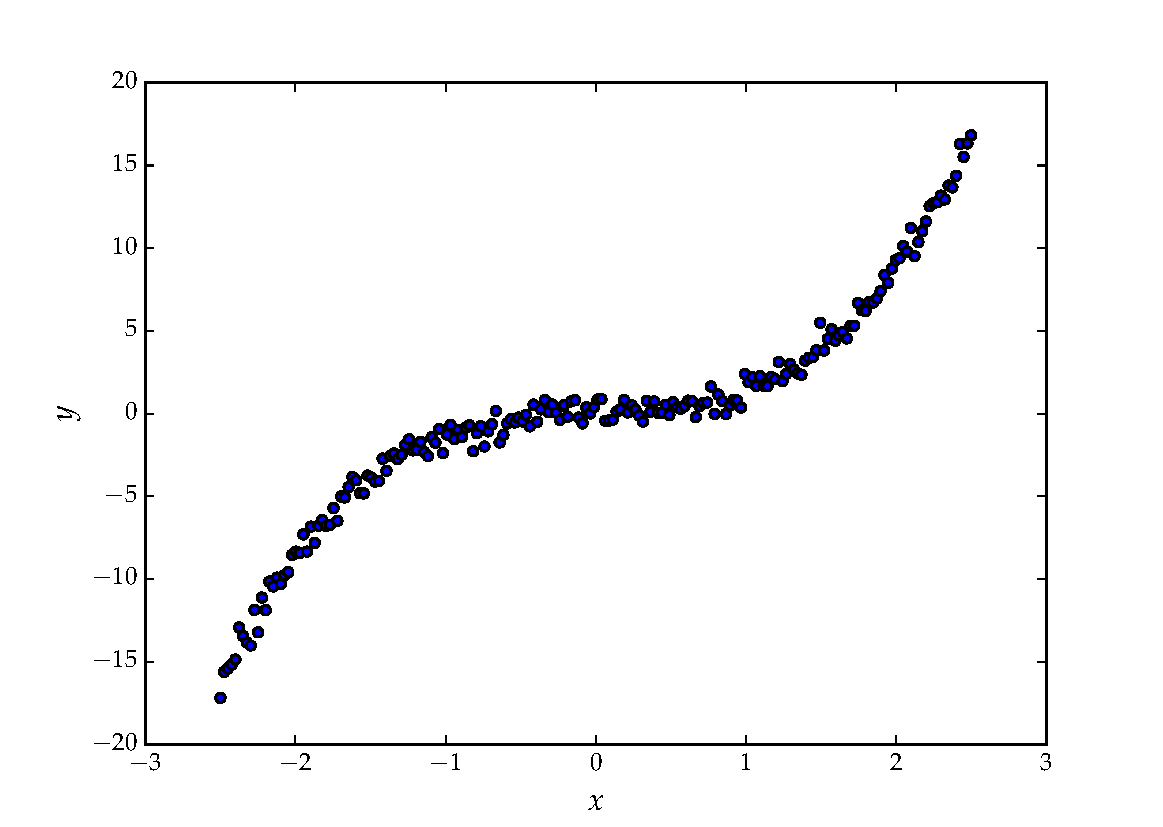
\includegraphics[trim={2em 2em 2em 2em}, clip]{linear_after_proj.pdf}}
    \caption{ Nonlinear relationship between $x$ and $y$}
    \end{figure}
    
\end{frame}

\begin{frame}

    \vspace{2em}
    Figure on following slide shows data after applying
    the transformation $\RR \ni x \mapsto \boldphi(x) := (x, x^3)^\T \in \RR^2$
    
    The
    plane drawn in the figure represents a linear function $\ell \colon
    \RR^2 \to \RR$
    
    \vspace{.7em}
    The composition $\ell \circ \boldphi$ has low approximation
    error
    
    The two figures illustrate how nonlinear data can become linear when
    projected into higher dimensions
    
\end{frame}

\begin{frame}

    \begin{figure}
    \centering
    \scalebox{.54}{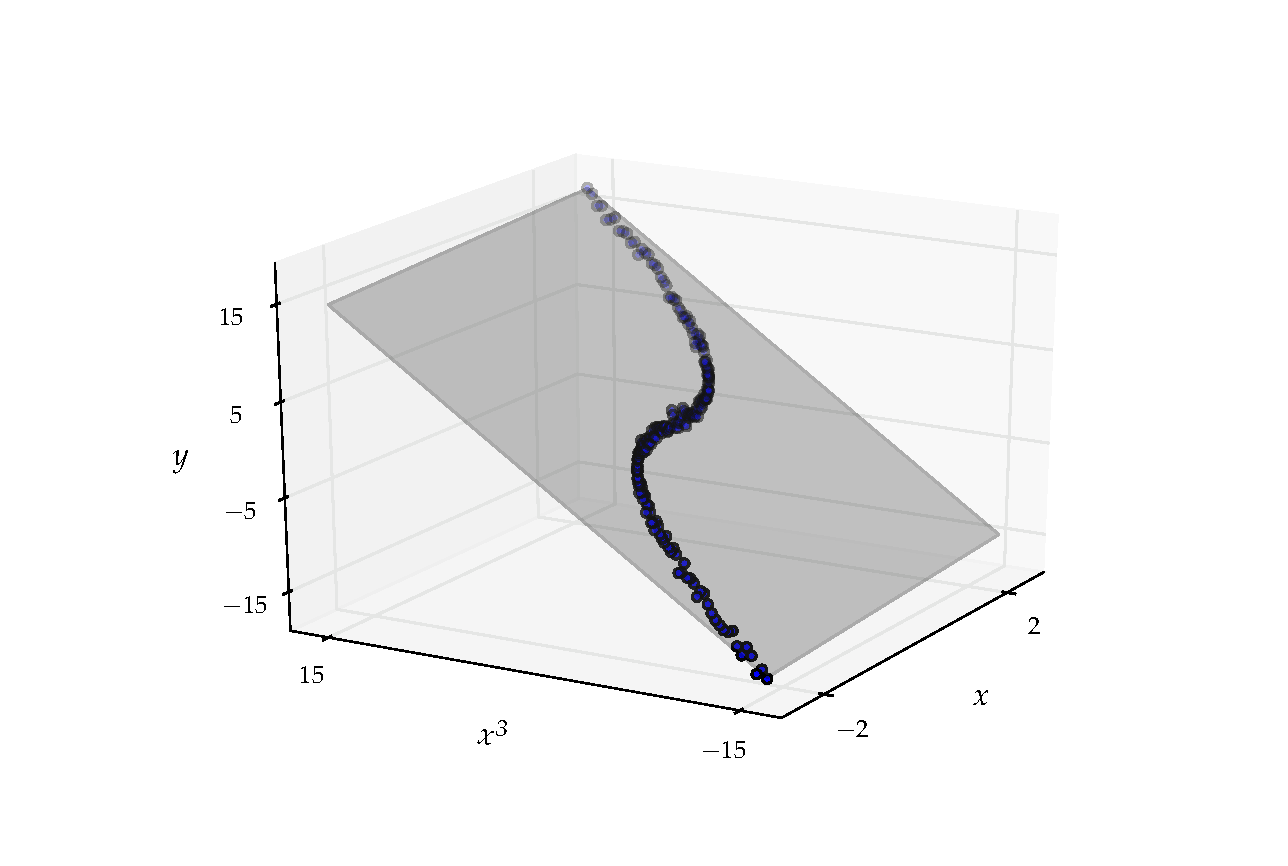
\includegraphics[trim={3em 2em 2em 5em}, clip]{linear_after_proj3d.pdf}}
    \caption{\label{f:lap3d} Approximate linearity after projecting the data to $\RR^2$}
    
\end{figure}

\end{frame}

\section{FWL Theorem}

\begin{frame}\frametitle{The Frisch--Waugh--Lovell Theorem}

    \vspace{2em}
    The Frisch--Waugh--Lovell (FWL) theorem yields an expression for an arbitrary
    sub-vector of the least squares estimator $\hboldbeta$ obtained by regressing
    $\boldy$ on $\boldX$
    
    \vspace{.7em}
    Continue with assumptions made already in the lecture
    
    Let $\boldy$ and $\boldX$ be given and let $\hboldbeta$ be the least squares estimator,
    as given by equation \eqref{eq:thelsqe} above
    
\end{frame}

\begin{frame}

    \vspace{2em}
    In addition, let $K_1$ be an integer with $1 \leq
    K_1 < K$, and let
    %
    \begin{itemize}
        \item $\boldX_1$ be a matrix consisting of the first $K_1$ columns of
            $\boldX$,
        \item $\boldX_2$ be a matrix consisting of the remaining $K_2 := K - K_1$
            columns,
        \item $\hboldbeta_1$ be the $K_1 \times 1$ vector consisting of the first
            $K_1$ elements of $\hboldbeta$.
        \item $\hboldbeta_2$ be the $K_2 \times 1$ vector consisting of the
            remaining $K_2$ elements of $\hboldbeta$,
        \item $\boldP_1 := \proj ( \colspace \boldX_1)$, and
        \item $\boldM_1 := \boldI - \boldP_1 =$ the corresponding residual
            projection
    \end{itemize}
    
\end{frame}

\begin{frame}

    \vspace{2em}
    \Thm
    [FWL theorem]
    \eqref{ET-t:fwl}
    The vector $\hboldbeta_2$ satisfies
    %
    \begin{equation*}
        \label{eq:fwle}
        \hboldbeta_2 
        = (\boldX_2^\T \boldM_1 \boldX_2)^{-1} \boldX_2^\T \boldM_1 \boldy
    \end{equation*}
    %
    For a proof, see ET page \pageref{ET-t:fwl}
    
\end{frame}

\begin{frame}

    \vspace{2em}
    The expression for $\hboldbeta_2$ in theorem~\ref{ET-t:fwl} can be rewritten as
    %
    \begin{equation}
        \label{eq:sxb2}
        \hboldbeta_2 
            = [(\boldM_1\boldX_2)^\T \boldM_1 \boldX_2]^{-1} (\boldM_1 \boldX_2)^\T \boldM_1 \boldy
    \end{equation}
    
    (see  exercise~\ref{ET-ex:cnxfwl})
    
    \vspace{.7em}
    The above formula gives us the following claim: there is
    another way to obtain $\hboldbeta_2$ besides just regressing $\boldy$ on
    $\boldX$ and then extracting the last $K_2$ elements
    
    We can also regress
    $\boldM_1 \boldy$ on $\boldM_1 \boldX_2$ to produce the same result

\end{frame}

\begin{frame}

    \vspace{2em}
    For intuition: consider the case where $\boldX_2$ is the single column 
    $\col_K \boldX$, containing the
    observations on the $K$th regressor
    
    Write $\boldX_1$ as $\boldX_{-K}$ to remind us
    that it stands for all columns of $\boldX$ expect the $K$th one, and
    similarly for $\boldM_1$
    
    \vspace{.7em}
    The least squares estimate $\hat \beta_K$ can be found by regressing 
    %
    \begin{equation*}
        \label{eq:resregy}
        \tilde \boldy 
        := \boldM_{-K} \boldy = \text{residuals of regressing $\boldy$ on
        $\boldX_{-K}$}   
    \end{equation*}
    %
    on
    %
    \begin{equation*}
        \label{eq:resregx}
        \tilde \boldx_K 
        := \boldM_{-K} \col_K \boldX 
            = \text{residuals of regressing
                $\col_K \boldX$ on $\boldX_{-K}$}   
    \end{equation*}
    

\end{frame}

\begin{frame}

    \vspace{2em}
    The two residual terms $\tilde \boldy$ and $\tilde
    \boldx_K$ can be thought of as the parts of $\boldy$ and
    $\col_K \boldX$ that are ``not explained by'' $\boldX_{-K}$
    
    Intuitively, the process for obtaining the least squares estimate $\hat
    \beta_K$ is:
    %
    \begin{enumerate}
        \item remove effects of all other regressors from $\boldy$ and
            $\col_K \boldX$, producing $\tilde \boldy$ and $\tilde
            \boldx_K$
        \item regress $\tilde \boldy$ on $\tilde \boldx_K$
    \end{enumerate}
    
    \vspace{.7em}
    Different from the process for obtaining the coefficient of 
    the vector $\col_K \boldX$ in a simple univariate regression:
    %
    \begin{enumerate}
        \item regress $\boldy$ on $\col_K \boldX$
    \end{enumerate}
    
\end{frame}

\begin{frame}

    \vspace{2em}
    Difference between the univariate least squares estimated coefficient of 
    the $K$th regressor and the multiple regression least squares coefficient:
    \begin{itemize}
        \item the
    multiple regression coefficient $\hat \beta_K$ measures the \emph{isolated
    relationship} between $x_K$ and $y$
        \item does not take into account indirect
    channels involving other variables
    \end{itemize}
    %
\end{frame}

\begin{frame}

    \vspace{2em}
    We can illustrate further with simulation.  Suppose
    %
    \begin{equation*}
        y = x_1 + x_2 + u  
        \quad \text{where} \quad
        u \iidsim \nN(0,1)
    \end{equation*}
    %
    Generate $N$ independent observations from this model 
    
    \vspace{.7em}
    Regress $y$
    on the observations of $(x_1, x_2)$
    \begin{itemize}
        \item coefficients for $x_1$ and $x_2$ will both be close to
    unity, provided $N$ is sufficiently large
    \end{itemize}
    
    Regress $y$ on $x_1$ alone
    \begin{itemize}
        \item coefficient for $x_1$ will depend on the relationship between $x_1$ and $x_2$
    \end{itemize}
 
\end{frame}

\begin{frame}
    \vspace{2em}
     For example:
        %
        \inputminted{r}{small_sim.R}
        
        Here the coefficient for $x_1$ is much larger than unity
        \begin{itemize}
            \item an increase in $x_1$ tends to have a large positive effect on $x_2$,
        which in turn increases $y$
        \end{itemize}
        
\end{frame}

\begin{frame}\frametitle{Simple Regression}

    \vspace{2em}
    Application of FWL Theorem: derive expression for the slope coefficient 
    in simple linear regression from the multivariate expression
    
    \vspace{.7em}
    Simple linear regression as special case of multivariate regression
    \begin{itemize}
        \item $\boldone$ is the first column of $\boldX$ and $K = 2$
    \end{itemize}
    
    The second column of $\boldX$ will be denoted by $\boldx$
    
    The least squares estimates are
    %
    \begin{equation*}
        \hat \beta_2 = \frac{\sum_{n=1}^N (x_n - \bar x)(y_n - \bar y)}
                        {\sum_{n=1}^N (x_n - \bar x)^2}
        \quad \text{and} \quad
        \hat \beta_1 = \bar y - \hat \beta_2 \bar x
    \end{equation*}
    
    where $\bar x$ is the sample mean of $\boldx$ and $\bar y$ is 
    the sample mean of $\boldy$
    
\end{frame}

\begin{frame}

    \vspace{2em}
    We can rewrite the slope coefficient $\hat \beta_2$
    %
    \begin{equation}
    \label{eq:sre1}
    \hat \beta_2 = 
    [(\boldx - \bar x \boldone)^\T(\boldx - \bar x \boldone)]^{-1}
    (\boldx - \bar x \boldone)^\T(\boldy - \bar y \boldone)
    \end{equation}
    %
    By the FWL theorem (equation~\ref{eq:sxb2})
    %
    \begin{equation}
        \label{eq:sre2}
        \hat \beta_2 
            = [(\boldM_c\boldx)^\T \boldM_c \boldx]^{-1} (\boldM_c \boldx)^\T \boldM_c \boldy
    \end{equation}

    here $\boldM_c$ is the residual projection associated with the linear
    subspace $S = \Span\{\boldone\}$
    
    \vspace{.7em}
    For this residual projection $\boldM_c$ and any $\boldz$,
    we have $\boldM_c \boldz = \boldz - \bar z \boldone$ --- RHS of
    (\ref{eq:sre1}) and (\ref{eq:sre2}) coincide
    
\end{frame}

\begin{frame}

    \vspace{2em}
    Generalize to the
    case where there are multiple nonconstant regressors
    
    Instead of one column $\boldx$ of observations on a
    single nonconstant regressor, we have a matrix $\boldX_2$ containing multiple
    columns, each a vector of observations on a nonconstant regressor
    
    \vspace{.7em}
    If the least squares estimate $\hboldbeta$ is partitioned into $(\hat \beta_1,
    \hboldbeta_2)$, then
    %
    \begin{equation*}
        \boldX \hboldbeta = \boldone \beta_1 + \boldX_2 \hboldbeta_2
    \end{equation*}
    
    
    Applying the FWL theorem, we can write
    $\hboldbeta_2$ as
    %
    \begin{equation*}
        \hboldbeta_2 
            = [(\boldM_c\boldX_2)^\T \boldM_c \boldX_2]^{-1} (\boldM_c \boldX_2)^\T \boldM_c \boldy
    \end{equation*}
    %
    where $\boldM_c$ is the residual projection  (Equation \eqref{ET-eq:pczm} in ET)
    
\end{frame}

\begin{frame}

    \vspace{2em}
    $\boldM_c \boldy$ is $\boldy$ centered around its mean
    
    $\boldM_c\boldX_2$ is a matrix formed by taking each column of
    $\boldX_2$ and centering it around its 
    
    \vspace{1em}
    .....in a least squares regression with an intercept, the
    estimated coefficients of the nonconstant regressors
    are equal to the estimated coefficients of a zero-intercept regression
    performed after all variables have been centered around their mean

\end{frame}

\begin{frame}\frametitle{Centered $R^{2}$}

    \vspace{2em}
    Several versions of
    $R^2$ reported in common regression packages
    
    One of these is so called
    centered $R^2$
    
    \vspace{.7em}
    The version we discussed so far will now be called
    uncentered $R^2$
    
    Why introduce alternative to uncentered $R^2$? 
    \begin{itemize}
        \item fails to be invariant to certain changes of units that involve
                addition or subtraction whenever
                $\boldX$ contains an intercept
        \item for e.g. actual inflation versus inflation in excess of a
                certain level, income versus income over a certain threshold, etc.
    \end{itemize}


\end{frame}

\begin{frame}

    \vspace{2em}
    Define centered
    $R^2$ 
    %
    \begin{equation*}
        \label{eq:crs}
         R_c^2 
         := \frac{\| \boldP \boldM_c \boldy \|^2}{\| \boldM_c \boldy \|^2}
         = \frac{\|  \boldM_c \boldP \boldy \|^2}{\| \boldM_c \boldy \|^2}
    \end{equation*}
    %
    (See ex.~\ref{ET-ex:crs} to prove equality)
    
    \vspace{.7em}
    Adding a constant to each element
    of $\boldy$ will have no effect on $R^2_c$ because $\boldM_c$ maps constant
    vectors to $\boldzero$ (see example~\ref{ET-eg:pvonepm})
    
\end{frame}

\begin{frame}

    Rewrite $R^2$ (ex.~\ref{ET-ex:cecrs}) as
    %
    \begin{equation*}
        \label{eq:cecrs}
        R_c^2 = \frac{ \sum_{n=1}^N (\hat y_n - \bar y )^2 }
                { \sum_{n=1}^N (y_n - \bar y )^2 }
    \end{equation*}
    
    \vspace{.7em}
    In the case simple regression, $R_c^2$ is a measure of correlation
    
    \begin{itemize}
        \item $R_c^2$ is equal to the square of the
    sample correlation between the regressor and regressand, as defined by
    Equation \ref{ET-eq:sampcorr} (shown in ex.~\eqref{ET-ex:crsicc})
    \end{itemize}
    
\end{frame}



\end{document}
